\chapter{Sviluppo}

\section{Progettazione del sistema}
L'obiettivo di questo stage è stato la creazione del sistema di controllo di un robot a guida differenziale che si integrasse con il framework ROS.
Innanzitutto è stata necessaria un'analisi dei requisiti, nella quale sono stati individuati i seguenti punti: 
\begin{itemize}
    \item Elaborazione dei dati degli encoder per ricavare l'odometria del robot.
    \item Controllo dei motori tramite un sistema di retroazione.
    \item Comunicazione bidirezionale con un computer di controllo.
\end{itemize}

Per l'ultimo punto è stato necessario studiare un sistema per poter integrare la comunicazione con il framework ROS, in particolare per poter utilizzare il Navigation Stack.
Lo stack di navigazione è molto semplice a livello concettuale. Esso riceve le informazioni riguardanti l'odometria e i dati dei sensori, e restituisce in output i comandi che il robot deve eseguire.

\begin{figure}[h]
    \centering
    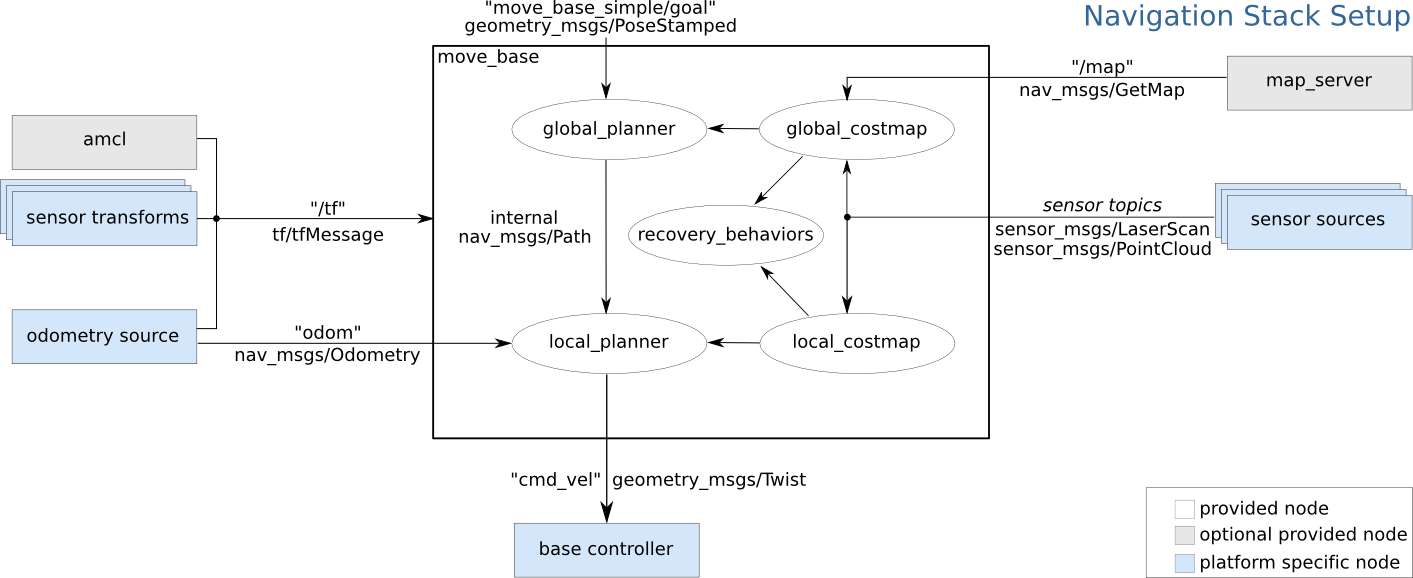
\includegraphics[scale=0.38]{images/navigation_stack.png}
    \caption{Lo schema dello stack di navigazione. Come mostrato nella legenda, i nodi in
bianco sono quelli già forniti, quelli in grigio sono opzionali e quelli in blu sono specifici per il singolo robot che devono essere implementati.}
  \label{fig:navigation_stack}
\end{figure}

\newpage
Come illustrato nella figura \ref{fig:navigation_stack} i messaggi da pubblicare, per quanto riguarda il sistema di controllo, sono messaggi di tipo \textit{nav\_msgs/Odometry} sul topic \textit{/odom} e i messaggi di tipo \textit{tf/Message} sul topic \textit{/tf}, e bisogna sottoscriversi ai messaggi di tipo \textit{geometry\_msgs/Twist} sul topic \textit{/cmd\_vel}. \\
Il messaggio \textit{Odometry} contiene le informazioni riguardanti la pose del robot nello spazio, prendendo come sistema di riferimento la prima posizione del robot ed è composto da:
\begin{itemize}
    \item Posizione espressa come \textit{x, y, z}
    \item Orientamento espresso come \textit{quaternion}
    \item Velocità lineare e velocità angolare attuali
\end{itemize}
Il messaggio \textit{tf} contiene le informazioni riguardanti pose del robot ed è necessario in quanto ci permette di rappresentare l'albero delle trasformazioni delle varie parti del robot, ovvero le posizioni relative delle varie parti come laser e altri sensori rispetto alla base mobile, chiamata \textit{base\_link} \\
Il messaggio \textit{geometry\_msgs/Twist} contiene le informazioni per far muovere il robot, nel caso di un robot a guida differenziale queste informazioni sono la velocità lineare sull'asse delle x, e la velocità angolare rispetto all'asse delle z.

Si è scelto di far gestire la parte relativa allo scambio dei messaggi ROS al computer principale, che comunica con la scheda di controllo tramite il modulo usb-seriale. 
Sono stati creati due nodi ROS, uno che si sottoscrive al topic \textit{/cmd\_vel} e trasmette i comandi alla scheda, e un nodo che riceve le informazioni relative alla velocità del robot, le elabora e pubblica i messaggi su \textit{/odom} e \textit{/tf}. \\
Il microcontrollore deve svolgere tre compiti: 
\begin{itemize}
    \item Gestire i loop di controllo PID per la gestione dei motori.
    \item Ricevere i comandi, ricavare i valori delle velocità dei motori e impostare quindi i setpoint dei controlli PID.
    \item Inviare i dati di odometria.
\end{itemize}

La trasmissione dei dati di odometria avviene periodicamente leggendo i dati degli encoder, mentre l'aggiornamento dei comandi da far eseguire ai motori avviene in modo asincrono ogni volta che il messaggio di comando viene ricevuto.

\section{Implementazione microcontrollore}
\subsection{Struttura del codice}
Lo scheletro del codice e l'inizializzazione delle periferiche sono stati generati tramite allo strumento STM32CubeMX. Il software è stato scritto in C++ per permettere un miglior riutilizzo del codice attraverso l'utilizzo delle classi.

\begin{figure}[H]
    \centering
    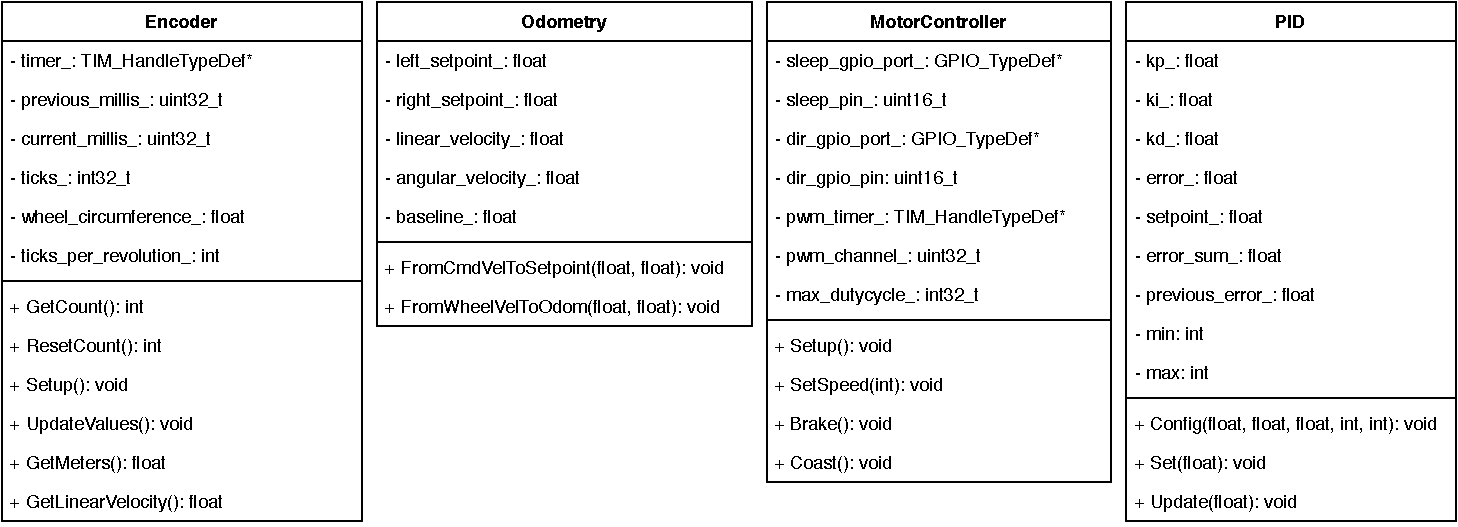
\includegraphics[scale=0.64]{images/uml_classes.pdf}
    \caption{Diagramma delle classi}
\end{figure}


\begin{figure}[H]
    \centering
    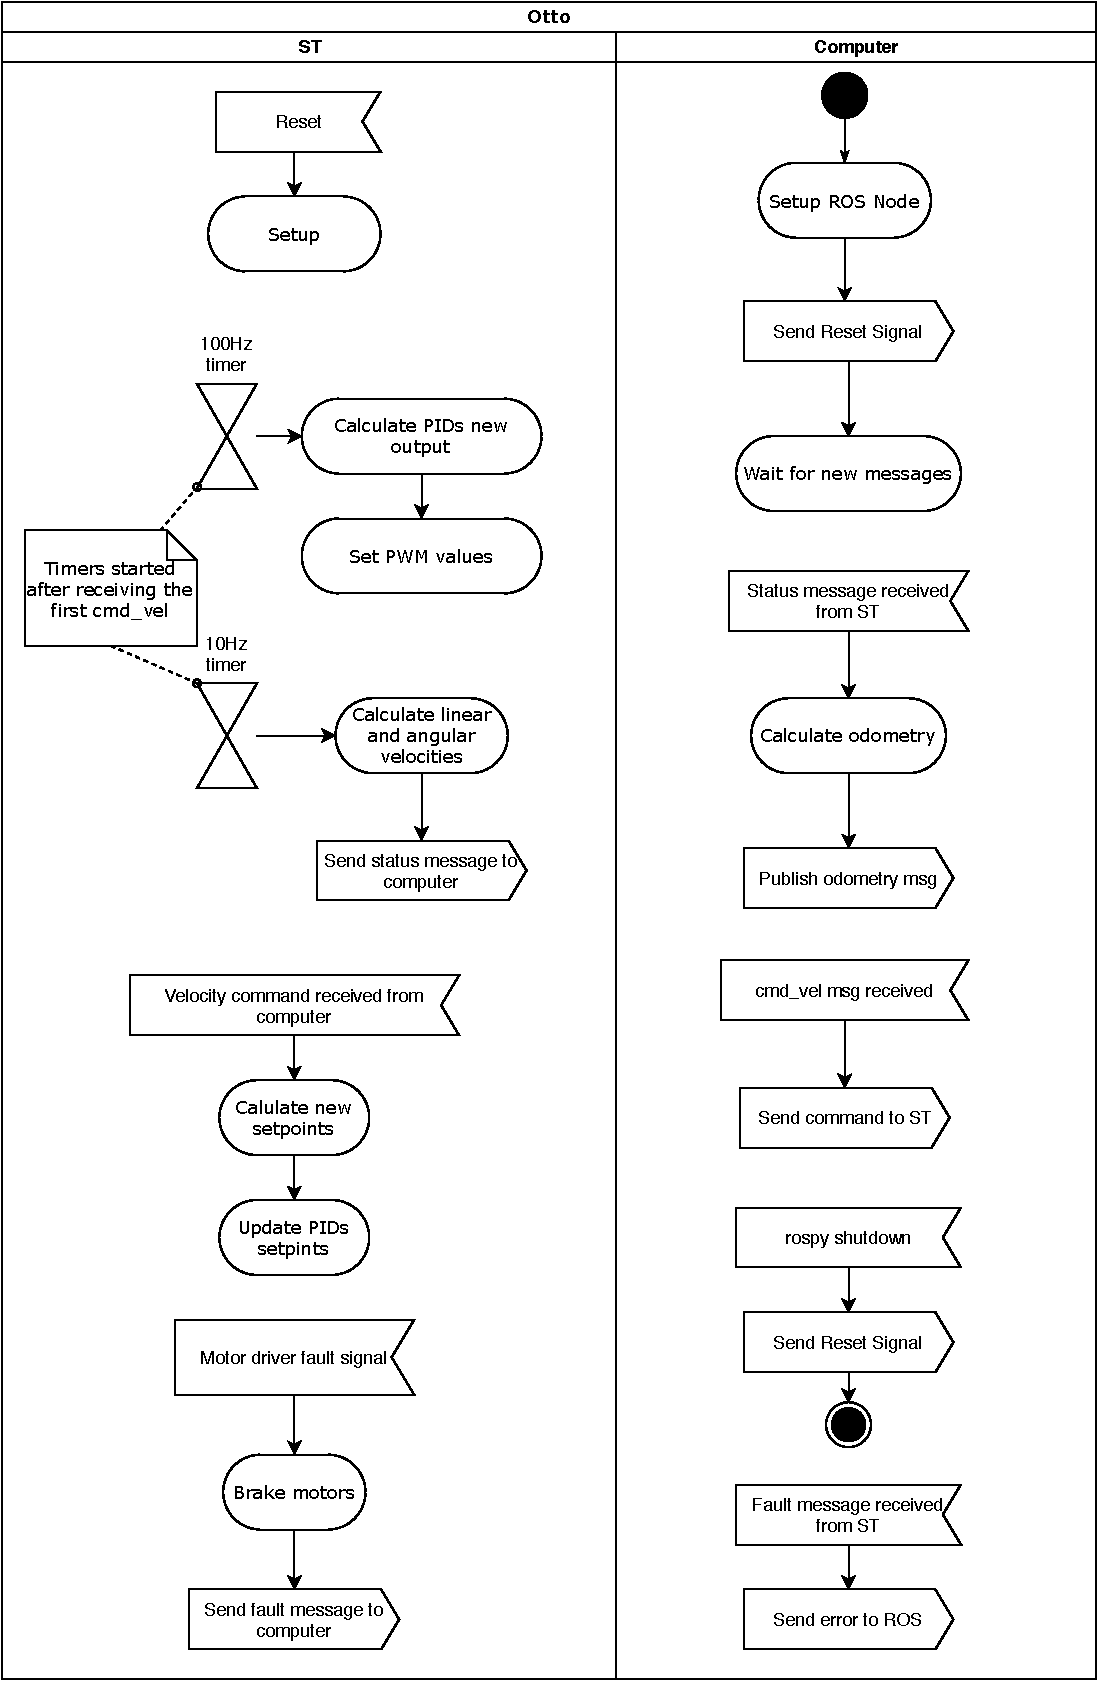
\includegraphics[scale=0.7]{images/uml_activities.pdf}
    \caption{Diagramma delle attività}
\end{figure}



\subsection{Lettura encoder}
\subsection{Controllo PID dei motori}
\cite{cross_pid}
\subsection{Comunicazione seriale con computer}
\section{Implementazione nodi ROS}
\section{Testing}
